\section{Fit Strategy and Validation}
\label{sec:fit_strategy}

The steps taken to validate the fitting approach for both the SVJ Fit strategy and the Discovery strategy will be outlined in the following sections. The signal region fits which comprise the final result will be presented in Chapter~\ref{ch:results}.

\subsection{SVJ Fit Strategy}
\label{subsec:fit_exclusion}

The ability of the five parameter fit function to capture the shape of the background is studied extensively, using data from the CR and VR. Signal injection tests are performed to determine the ability of the fit to recover and quantify any SVJ signal excess. Estimates of the expected sensitivity and the ability to set upper limits on the cross section of the signal process are also verified.\par
%Results: An overview of the final fit setup including the final discriminating variables(s), the (SR/CR) regions to be included in the fit and the floating normalization parameters. 
%Some rough first expected limits/discovery sensitivity plots are useful if you have them but not necessary. In this case the binning of the final variable(s) and the systematics smoothing/pruning should be indicated.

The fit results are primarily evaluated by their $p$-value, which dictates the probability of observing the given data spectrum given the fit hypothesis.
A higher $p$-value is an indication of better agreement between the data and the fitted shape. 
The $\chi^2$/d.o.f. (or chi-sqaure per degrees of freedom, shown as just ``$\chi^2$'' or ``x'') is also presented.
The $\chi^2$ is checked to make sure it is not substantially larger or smaller than 1.0. 
$\chi^2$ values close to 1.0 indicate that the fit is able to capture the data without overfitting.
For each fit, the pattern of the residuals is also shown.
The residual is calculated as the difference between the observed data in a bin and the fit estimation for the bin, divided by the statistical uncertainty, indicating the significance of the deviation from the fit estimation.

%------------------------------------------------- 
\subsubsection{Background Only Fits}
\label{subsec:fit_bkgonly}

The background fit polynomial is validated using the original data from the CR and VR, and pseudo-data generated from the CR.

The nature of the functional fitting method allows the fit to easily adapt to changes in slope of a smoothly falling distribution.
Thus validation of the fit can be performed in data using the CR and the VR distributions to model the expected behavior in the SR, despite the expected differences in slope of the \mt~distribution illustrated in Figure~\ref{fig:crvrsr_mt}.
Figure~\ref{fig:bkgfit_data_fullstats} shows the a successful fit performed on the full statistics CR and VR regions.
The \mt~spectrum is fit in 90 bins of width 50 GeV. 
For the purposes of this analysis, any converged fit with a $p$-value > 0.05 is considered successful. 

\begin{figure}[!htbp]
\centering
   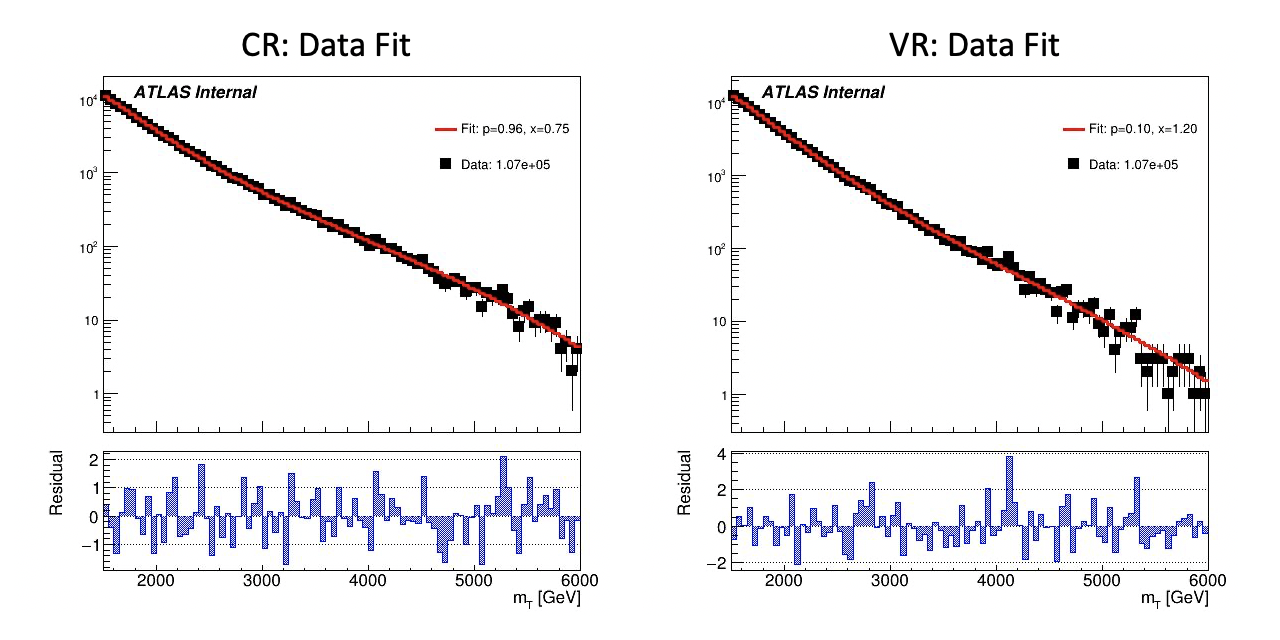
\includegraphics[width=0.8\textwidth]{figures/stats/bkgfit_data_fullstats}
    \caption{Background-only \mt~fits using data in the full statistics CR and VR regions. The fit is observed to converge with $p$-value > 0.05. The distribution of residuals is reasonably flat. The number of events in the data histogram, $p$-value and $\chi^2$ value (x) are reported in the legend. 
    \label{fig:bkgfit_data_fullstats}}
\end{figure}

Table~\ref{fig:postfit_param_pfn} shows the post-fit values of the fit parameters and their uncertainties for each fit. Fits of the MC background in the CR, VR, and SR were also performed and observed to be successful. These fit are available in Appendix~\ref{app:mcfit}. 
\begin{table}[!htbp]
\centering
   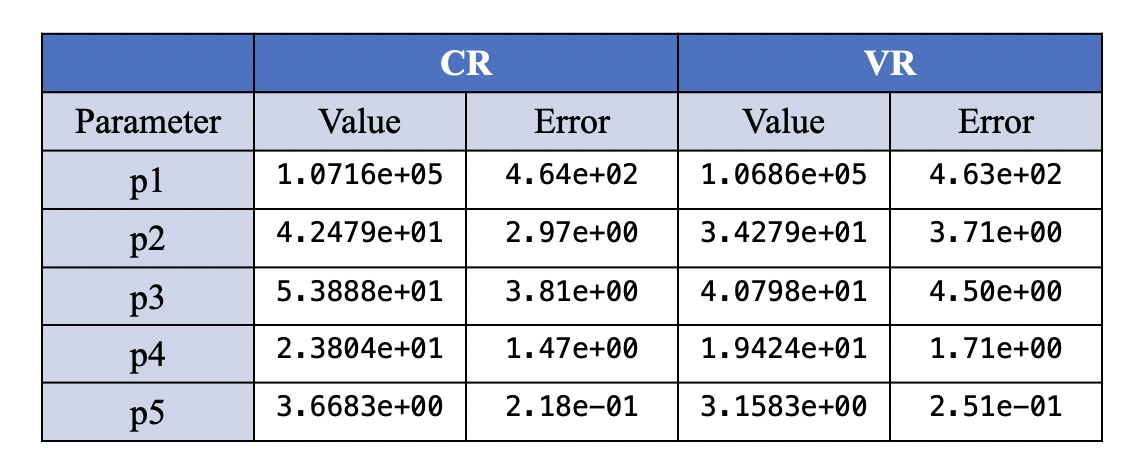
\includegraphics[width=0.75\textwidth]{figures/stats/postfit_param_pfn}
    \caption{Post-fit parameters for the PFN CR and VR. $p1$ can also be considered $N_{bkg}$ or the normalization factor.
    \label{fig:postfit_param_pfn}}
\end{table}

To further validate the fit stability of the fit against potential statistical fluctuations, \textit{pseudo-data} (also known as \textit{toy data}) are created from the CR data distribution. 
The pseudo-data is created following an \textit{Asimov} prescription \cite{asimov}, using a template to generate a set of toys representing different possible statistical fluctuations.
When studied as a group, the performance of the pseudo-data collection represents the range of possible behavior for an unknown distribution, such the the SR data, given its statistical uncertainties.

The template used to generate the pseudo-data is a \textit{smoothed} and \textit{scaled} version of the CR. 
The smoothing applied follows the procedure for functional decomposition described in Ref.~\cite{edgar2018functional}.
Figure~\ref{fig:smoothing} shows the impact of smoothing on the source data distribution in the CR.
\begin{figure}[!htbp]
\centering
   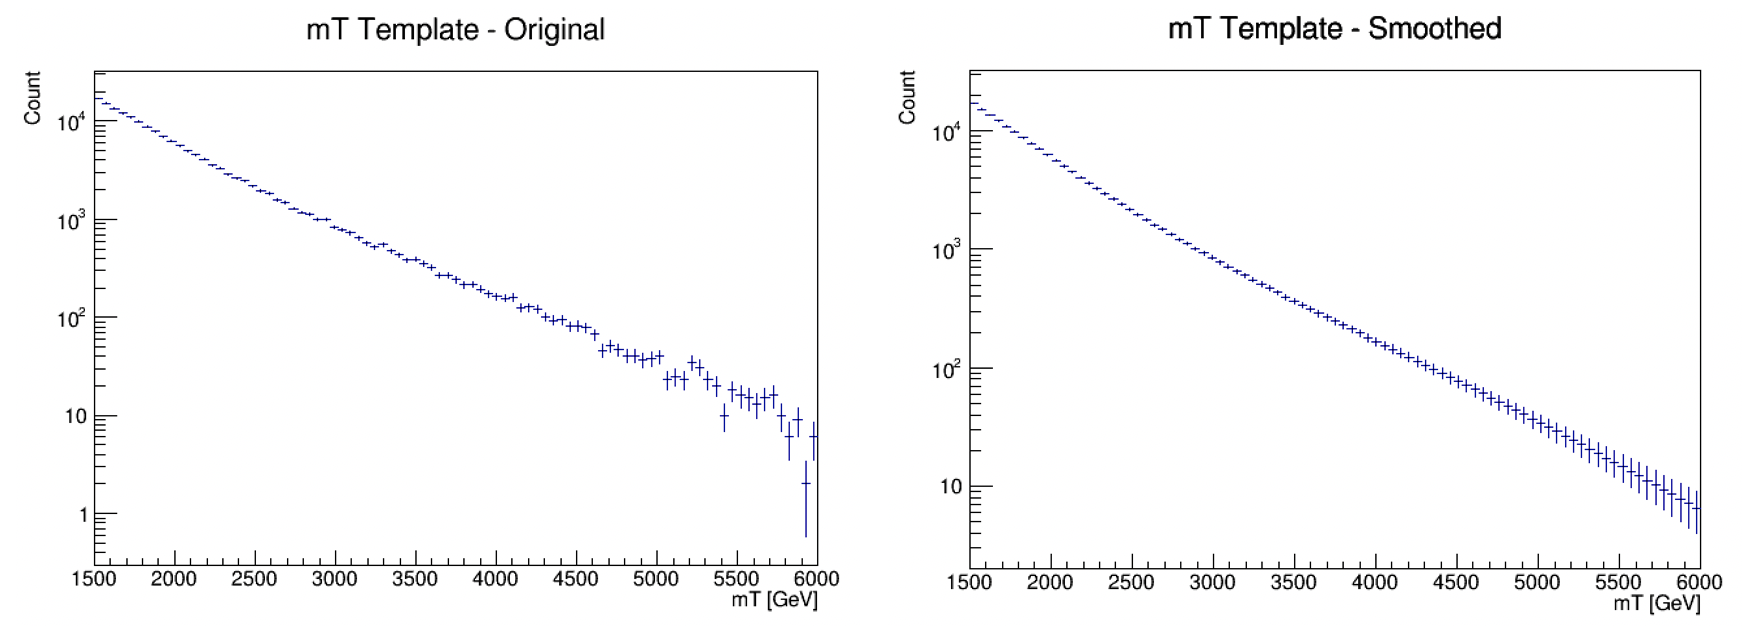
\includegraphics[width=0.95\textwidth]{figures/stats/smoothing}
    \caption{\mt~distribution in the data CR, before (left) and after (right) smoothing.
    \label{fig:smoothing}}
\end{figure}

The scaling adjusts the statistics of the smoothed template to the expected statistics of the SR.
Recall Figure~\ref{fig:crvrsr_2d}, which illustrates that the statistics (or number of events) in the CR and the VR are almost 3x the expected statistics of the SR.
The polynomial fitting strategy is sensitive to the statistics of the fitted template, so its performance can vary substantially depending on the statistical power of the fitted distribution.
To simulate this, the smoothed template is scaled to the expected statistics of the SR.
Toys are then generated from the smoothed distribution, by varying each bin within its statistical uncertainty according to a Poisson distribution. 
Each toy has the same statistical power as the SR, within statistical uncertainly.

Figure~\ref{fig:bkgfit_data} shows example fits to three such toy datasets.
Figure~\ref{fig:asimov_hist} shows the resulting p-values after an ensemble of 100 Asimov pseudo-datasets are each individually fit. 
This test determines the likelihood of exceptionally good (high $p$-value) or poor (low $p$-value) fits due to randoms statistical fluctuations in the data. 
A flat distribution is observed, indicating that the data is compatible with the background fit function. 
By definition, if the null hypothesis is true (meaning the data is compatible with the background expectation) there is a 10\% chance of a $p$-value less than 0.10, etc.
This leads to a flat distribution of $p$-values across many tests.

\begin{figure}[!htbp]
\centering
   %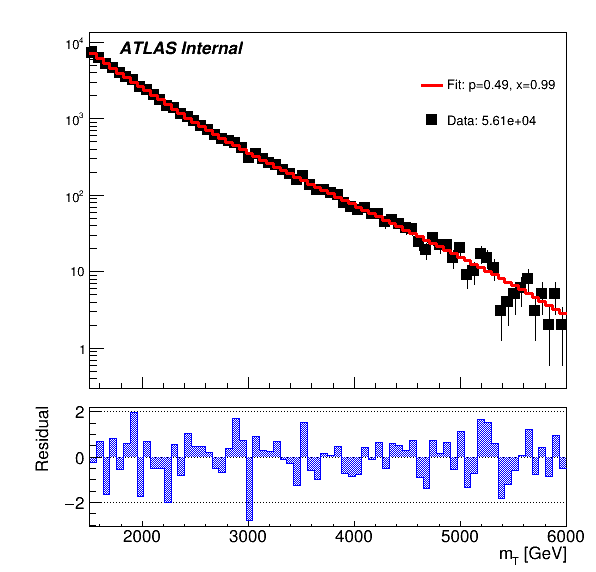
\includegraphics[width=0.32\textwidth]{figures/stats/dataDSfiveParFitChi2_CR0.png}
   %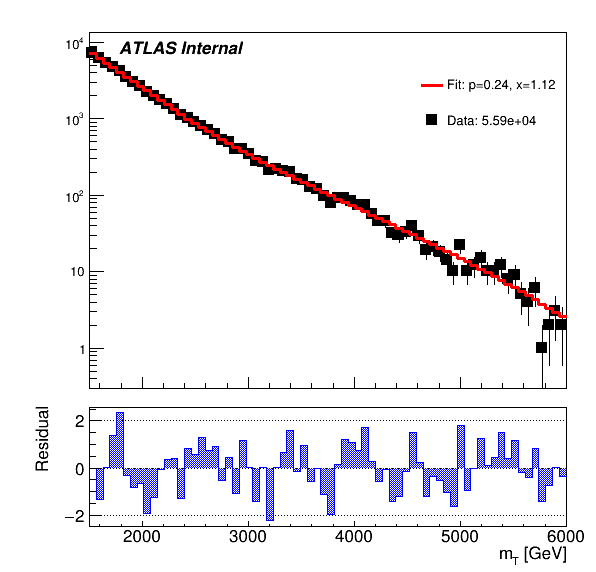
\includegraphics[width=0.32\textwidth]{figures/stats/dataDSfiveParFitChi2_CR1.png}
   %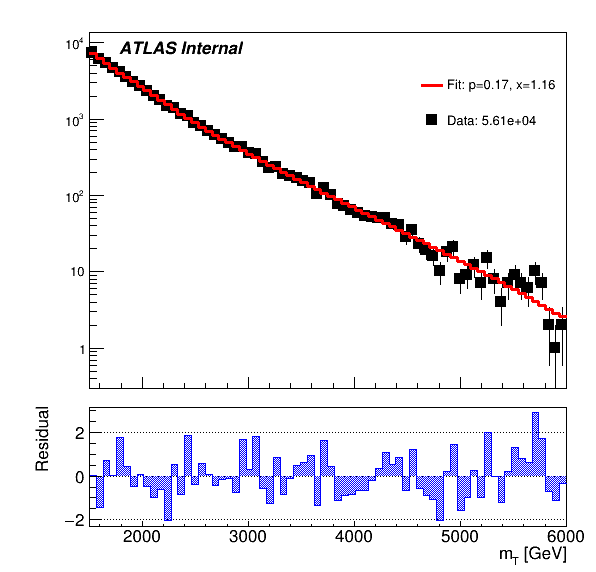
\includegraphics[width=0.32\textwidth]{figures/stats/dataDSfiveParFitChi2_CR2.png}
   %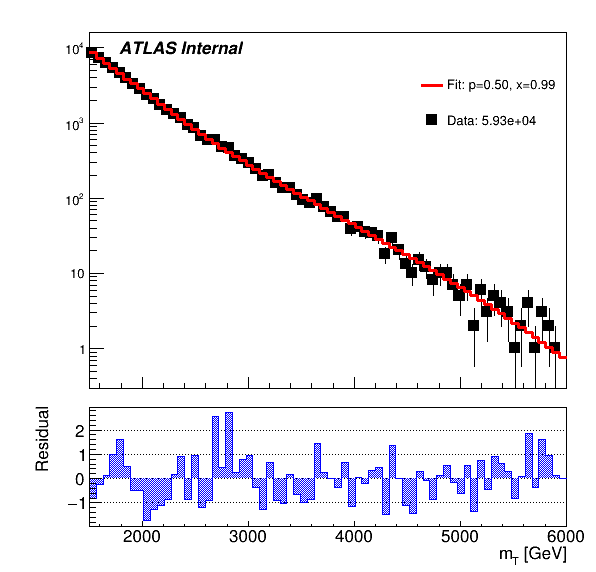
\includegraphics[width=0.32\textwidth]{figures/stats/dataDSfiveParFitChi2_VR0.png}
   %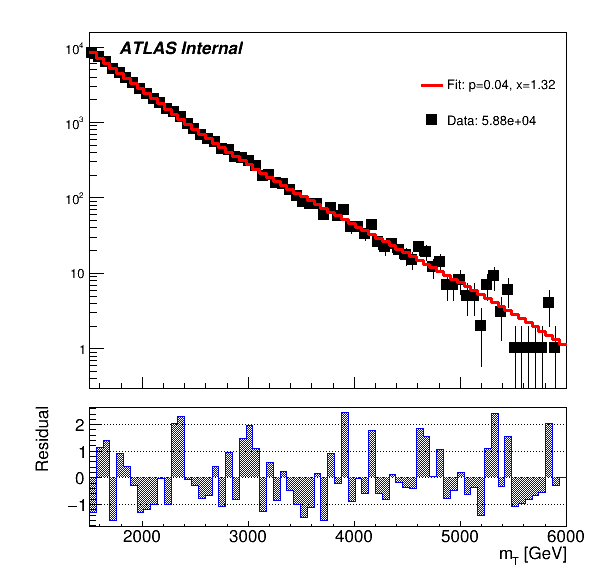
\includegraphics[width=0.32\textwidth]{figures/stats/dataDSfiveParFitChi2_VR1.png}
   %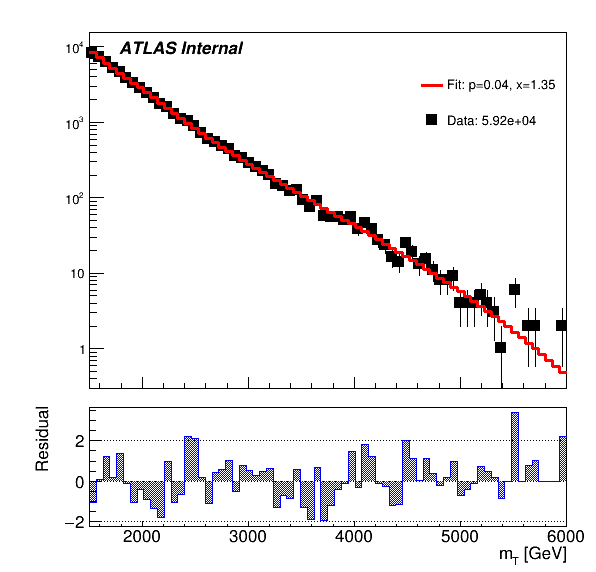
\includegraphics[width=0.32\textwidth]{figures/stats/dataDSfiveParFitChi2_VR2.png}
   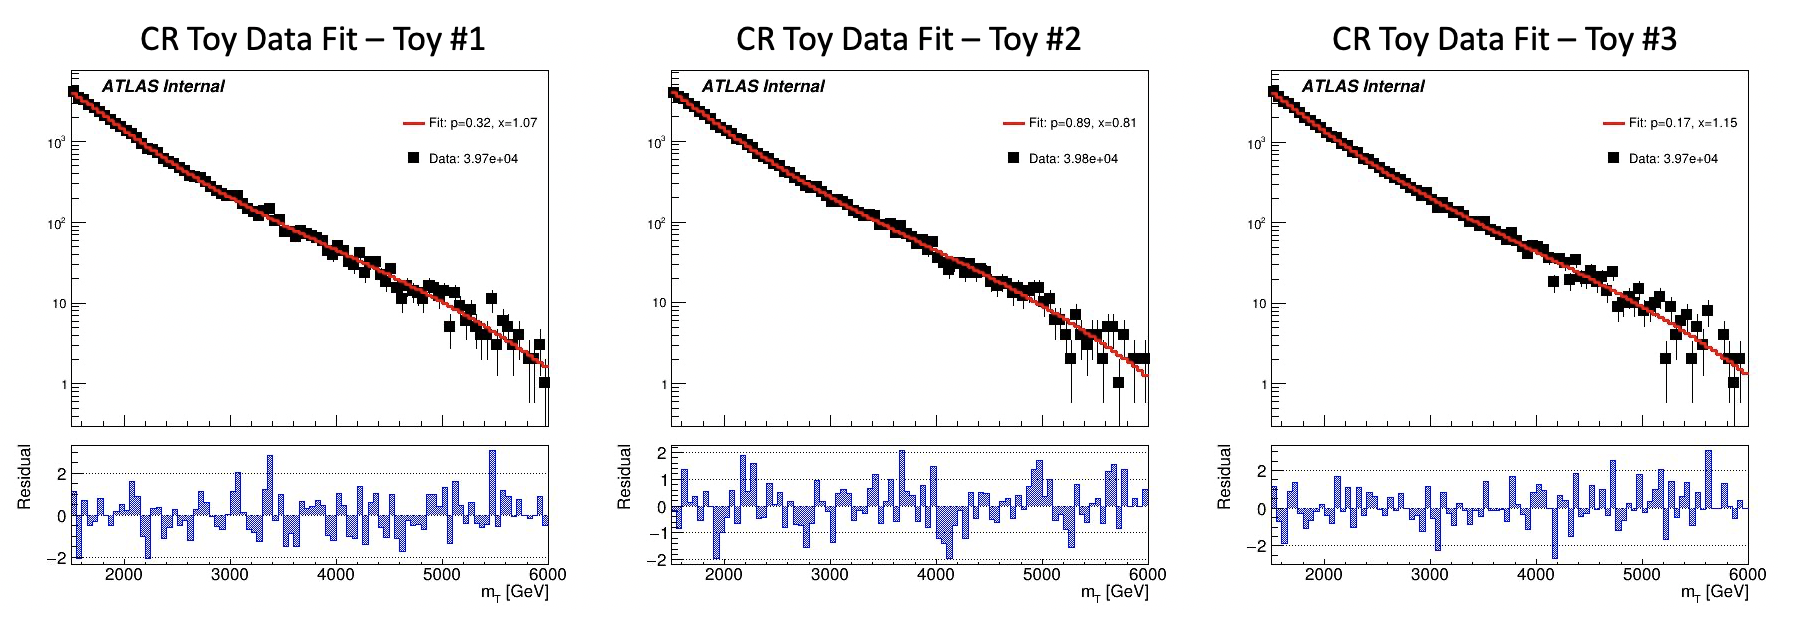
\includegraphics[width=0.97\textwidth]{figures/stats/bkgfit_data_cr}
    \caption{Background-only \mt~fits using pseudo-data from the CR template. All three fits are seen to successful converge, with varying $p$-values. The distribution of residuals is reasonably flat for all three fits.
     \label{fig:bkgfit_data}}
\end{figure}

\begin{figure}[!htbp]
\centering
   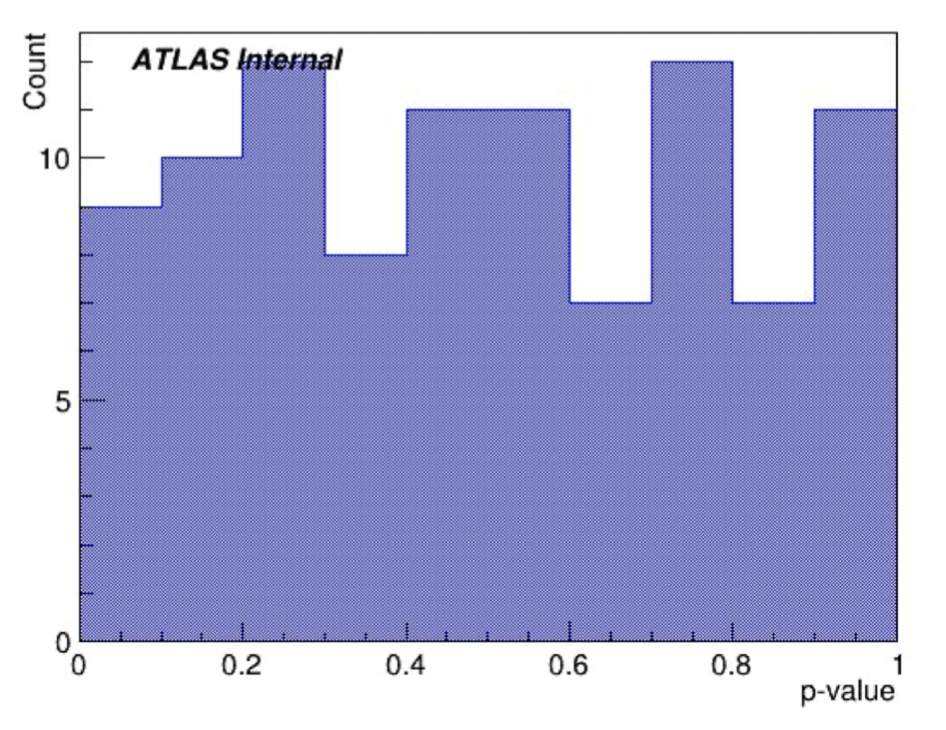
\includegraphics[width=0.6\textwidth]{figures/stats/asimov_cr_hist}
    \caption{$p$-value histograms from 100 fits to Asimov data in the CR. The even distribution of $p$-values between 0 and 1 indicates that the behavior of the fit is healthy. 98 $p$-values are shown, as two are excluded due to fits that did not converge on the first try. These fits later converged after the initial parameters were adjusted. %, demonstrating a flat shape across p-value.
    \label{fig:asimov_hist}}
\end{figure}

\clearpage
%------------------------------------------------- 
\subsubsection{Signal + Background Fits}
\label{subsec:fit_splusb}

Figure~\ref{fig:splusb_sigInj} shows an example of an injected signal into the exclusion region \mt~spectrum, and the ability of the fit framework to accurately fit the number of signal events.
\begin{figure}[!htbp]
\centering
   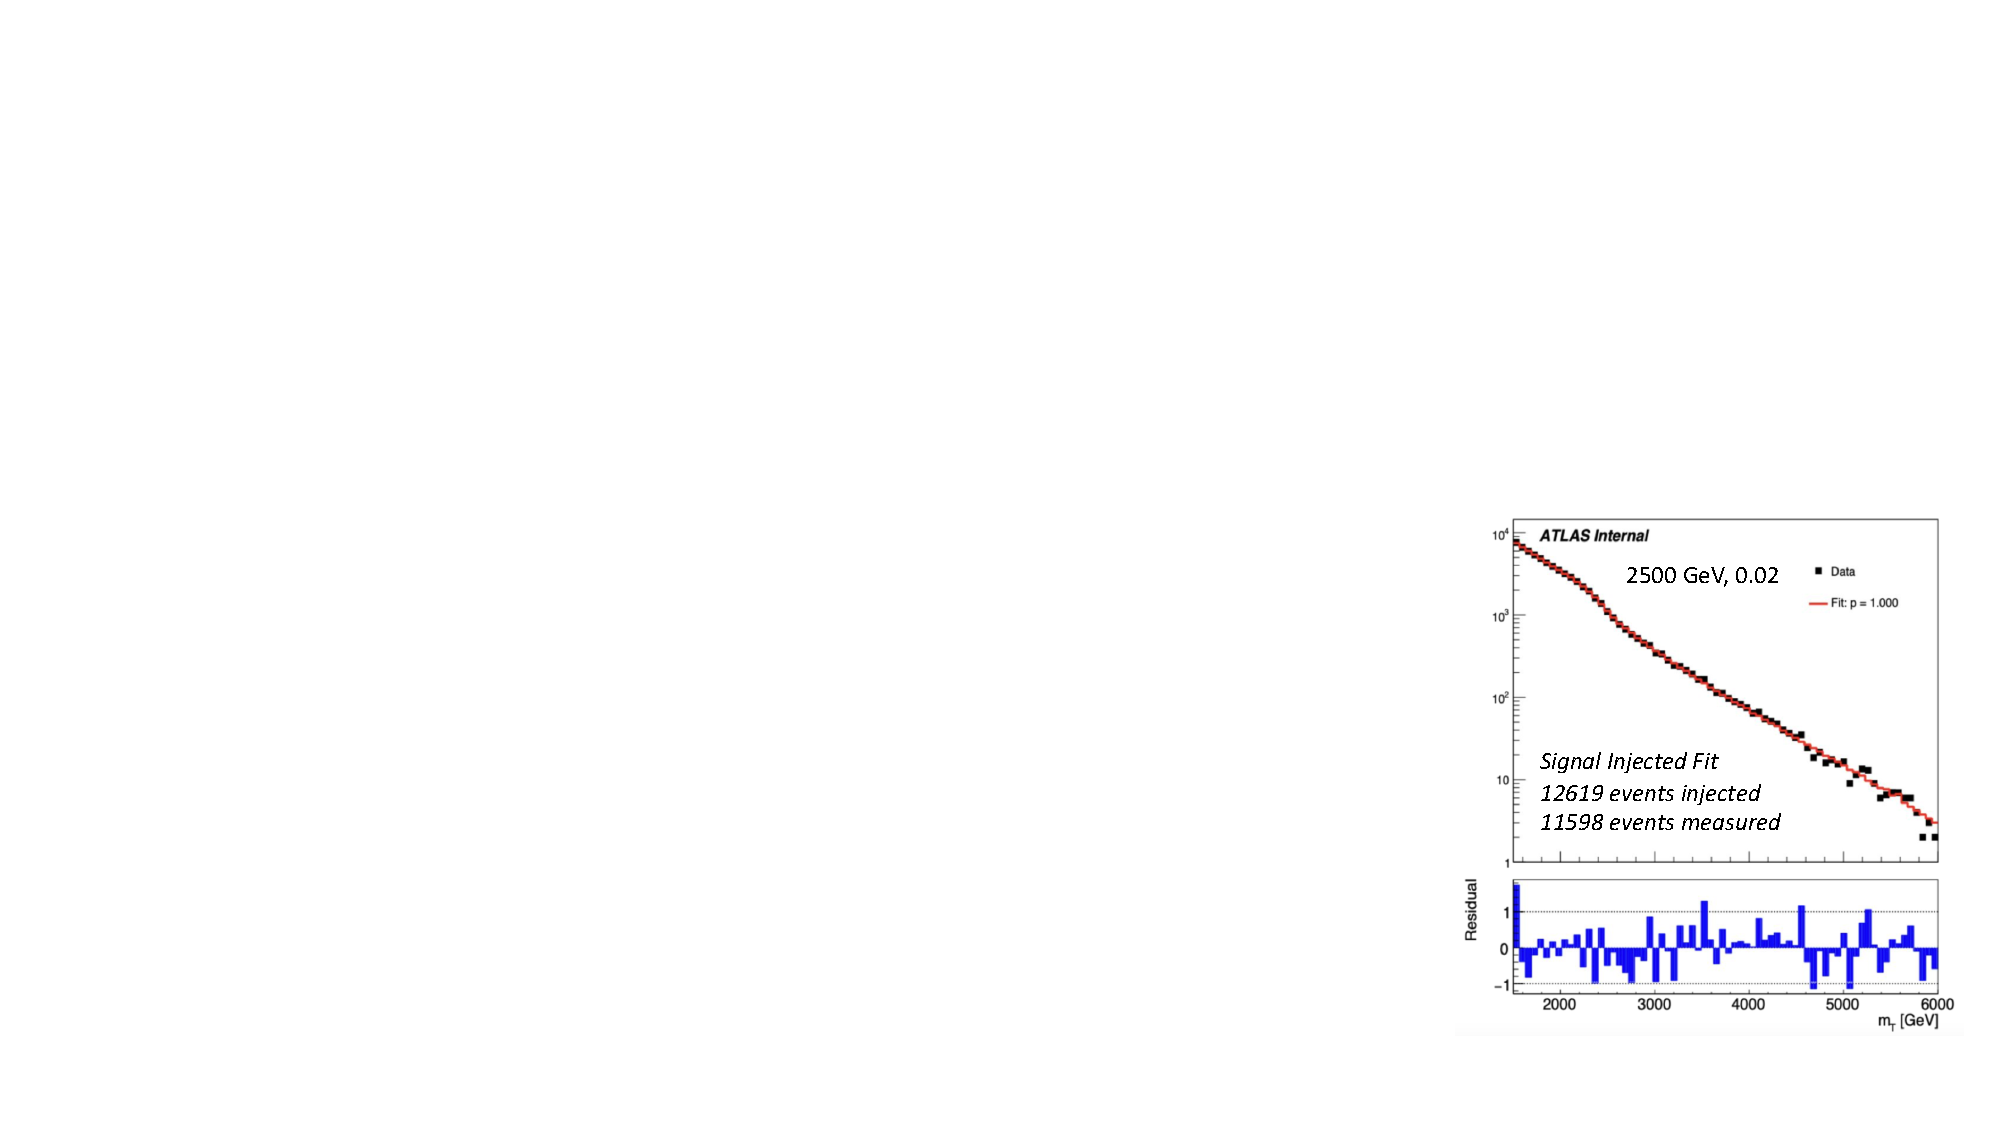
\includegraphics[width=0.6\textwidth]{figures/stats/splusb_sigInj}
    \caption{Example S+B fit on a background \mt~spectrum with injected signal from the point (4000 GeV, \rinv=0.2). The shape of the injected signal can be seen in Figure~\ref{fig:mt_mass}. The ability of the s+b fit to capture the shape of the signal and accurately measure the amount of injected signal is observed.
    \label{fig:splusb_sigInj}}
\end{figure}

Signal injection tests demonstrate the a linear relationship between the amount of signal injected and the amount of signal measured by the fit.
The signal injection tests are performed in Asimov datasets to counter the impact of statistical fluctuations in any given template.
50 Asimov trials are run for all signal points across $Z'$ mass and \rinv.

%Bias within the Asimov signal injection test could indicate a lack of sufficient normalization uncertainties on the signal model. 
%In the event of systematic mismeasurement in signal injection, the spurious signal uncertainty as derived from Loose-not-tight or additional uncertainties will be considered.

Figure~\ref{fig:siginj_asimov} provides the results of these tests. 
The uncertainty of the measurement varies according to the $Z'$ mass, due to the larger relative background for lower mass points. 
However, a strong linear relationship between amount of signal injected and amount of signal measured is observed for all signal points, which is the key feature.
The dashed lines illustrate the linear relationship, showing that for all points, the amount of signal measured increases as more signal is injected.
The variation in the y-intercept of the fitted dashed lines and the exact number of signal events measured for each injection level is not as significant as the overall linear behavior which is exhibited.
\begin{figure}[!htbp]
\centering
   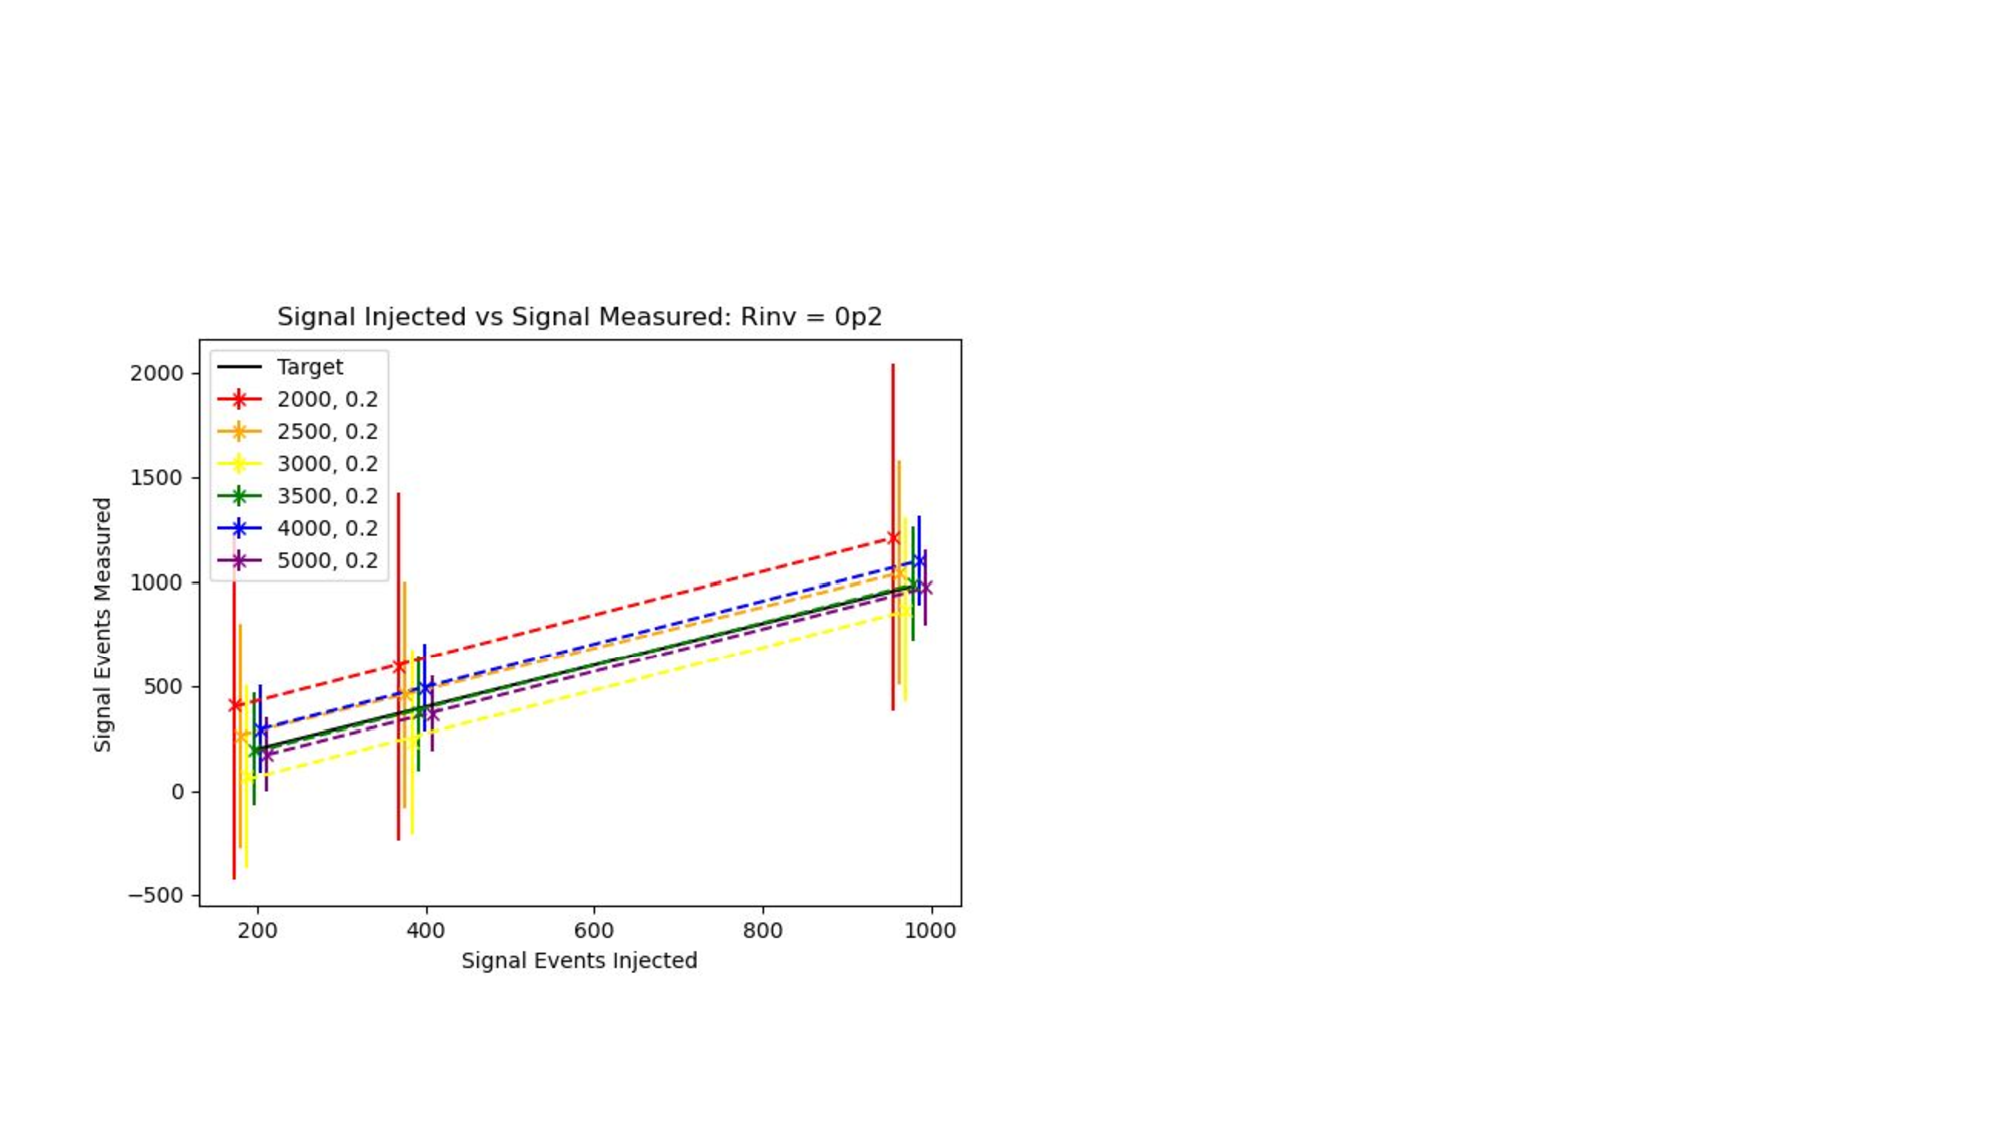
\includegraphics[width=0.45\textwidth]{figures/stats/siginj_asimov_02}
   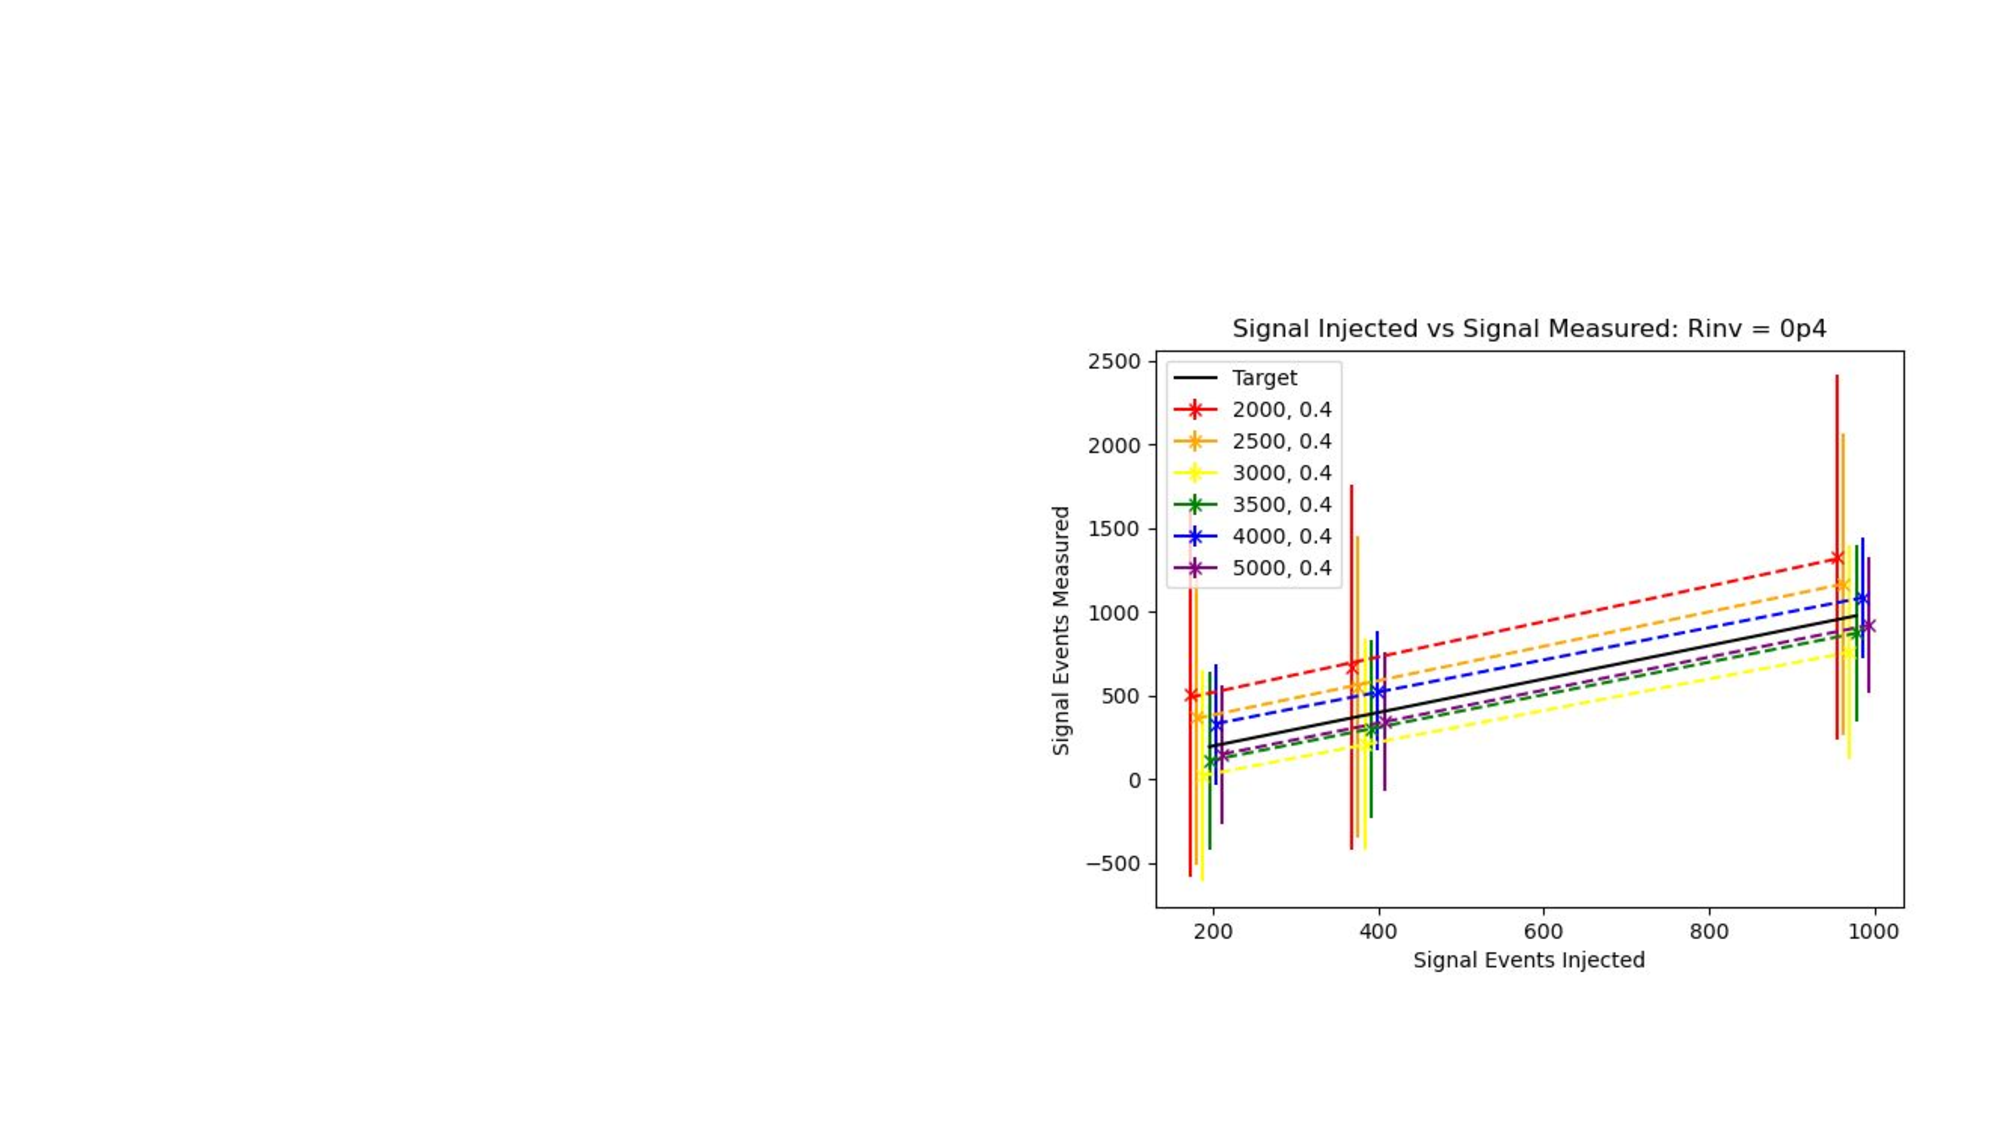
\includegraphics[width=0.45\textwidth]{figures/stats/siginj_asimov_04}
   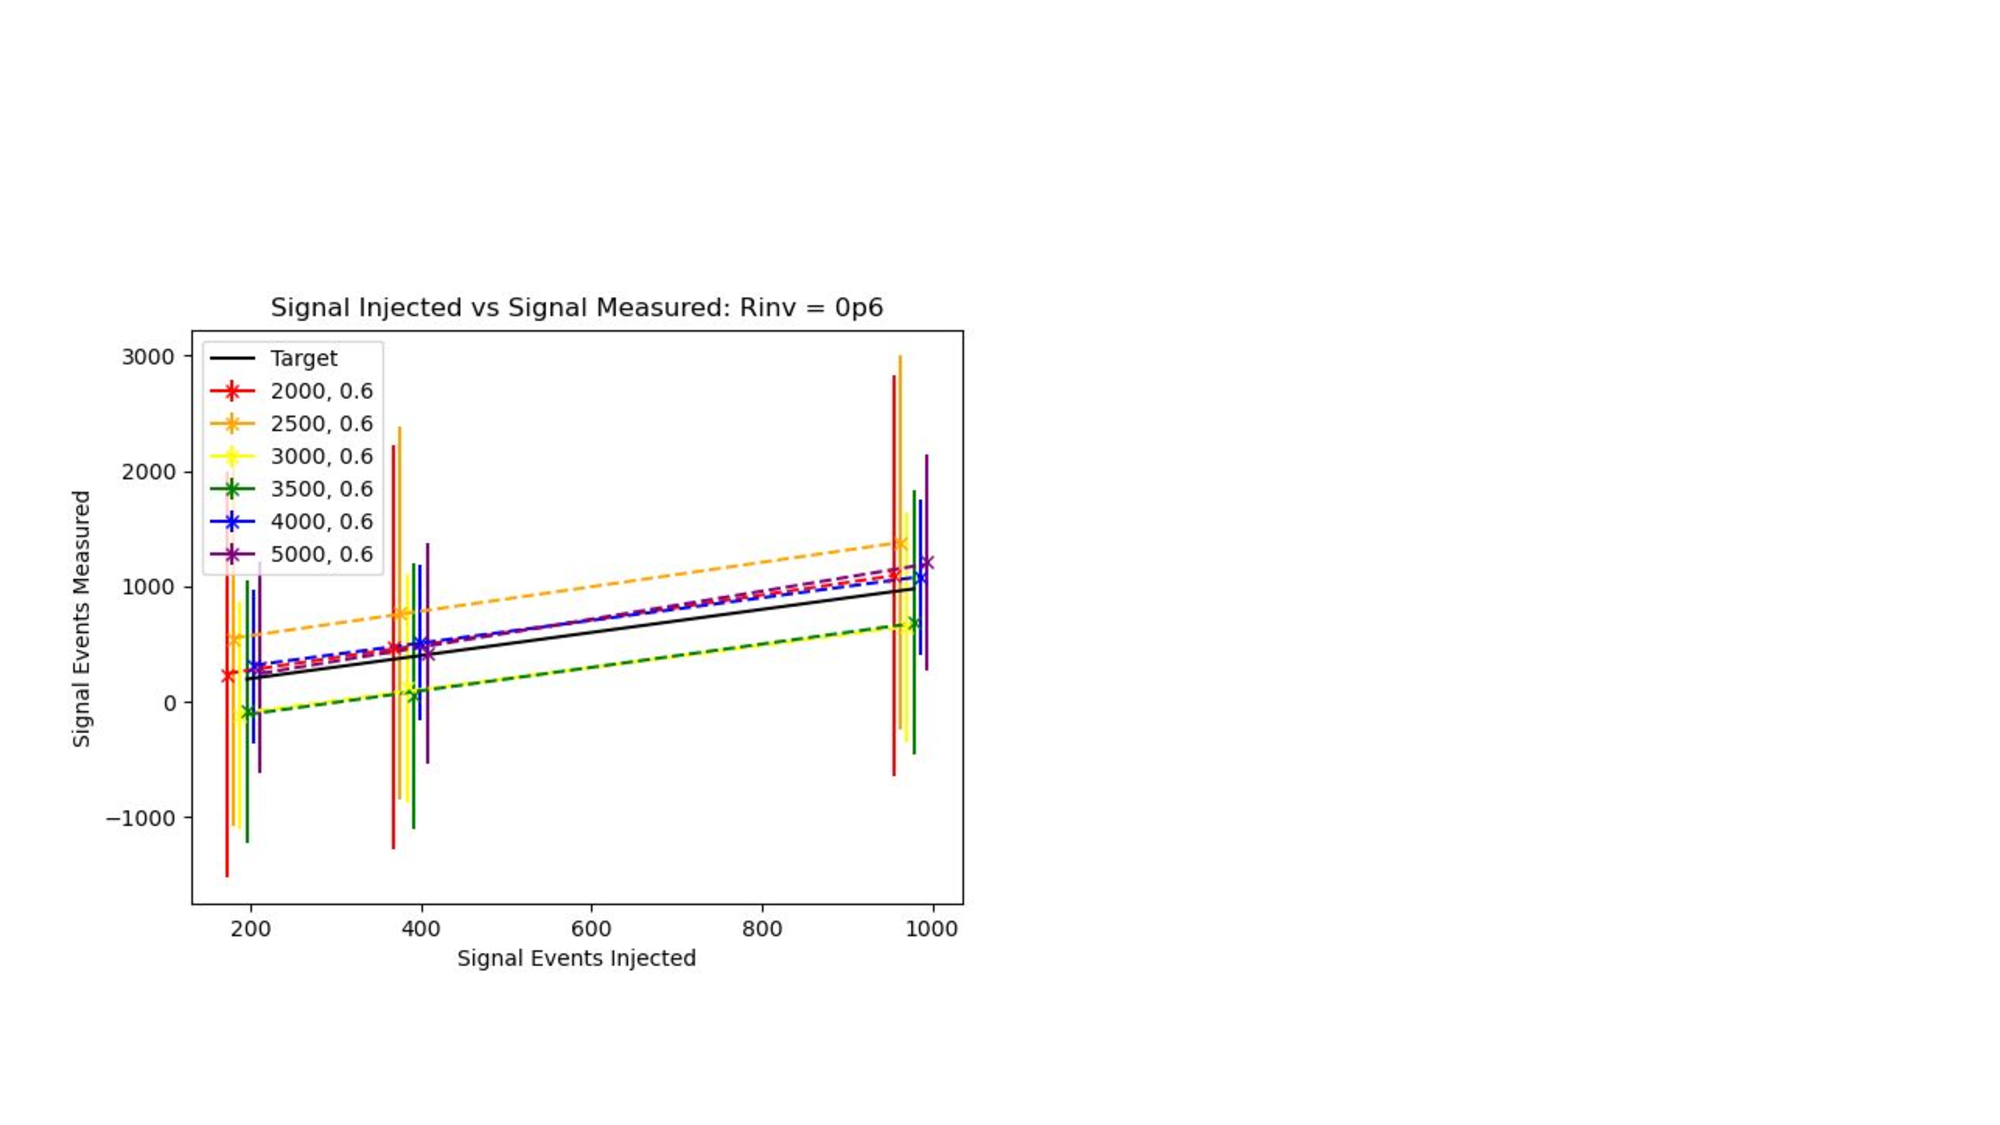
\includegraphics[width=0.45\textwidth]{figures/stats/siginj_asimov_06}
   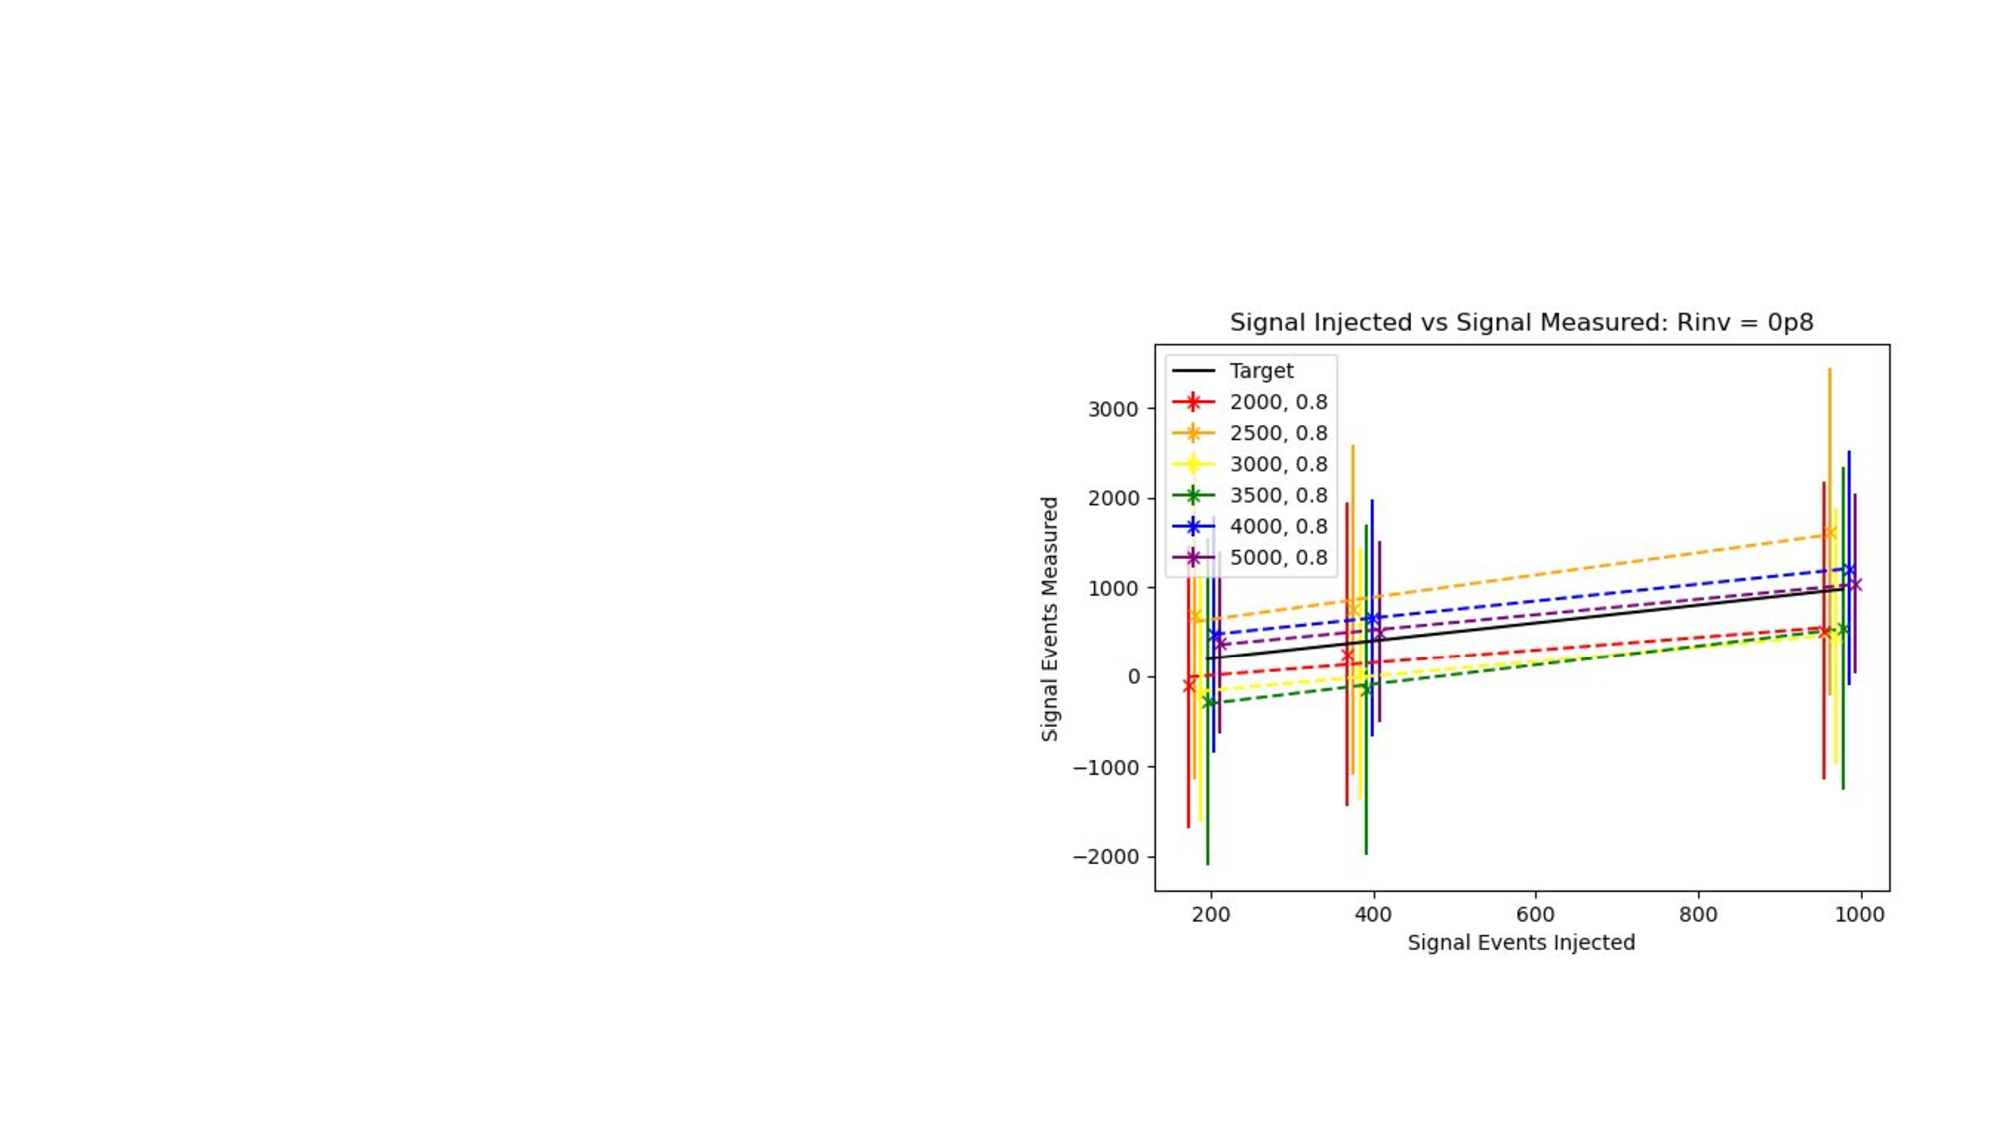
\includegraphics[width=0.45\textwidth]{figures/stats/siginj_asimov_08}
   \caption{Measured signal at a variety of injected values (1x, 2x, and 5x $\sqrt{b}$), for all signal points in the grid, \rinv~= 0.2 (top left), 0.4 (top right), 0.6 (bottom left), and 0.8 (bottom right). The x-axis values are slightly shifted from their true value so that all points can be viewed simultaneously. The error bars indicate the standard deviation of the number of fitted events across the 50 Asimov experiments. While the errors are large for some points, the strong linear relationship of the means, illustrated by the dashed lines, is the key feature.
%he requirement relative to $\sigma_{\text{fit}}$ is met for every signal point and injected signal size, thus satisfying the OR criteria from Equation~\ref{eq:spursig}.
    \label{fig:siginj_asimov}}
\end{figure}

\clearpage
%------------------------------------------------- 
\subsubsection{Expected Sensitivity}
\label{subsec:fit_expsens}

Limits on the signal process are obtained by determining the cross section of the signal process $Z'\rightarrow q_D \bar{q_D}$ that can be excluded at the 95\% Confidence Level (CL). 
\textit{Limits} refer to determining the maximum (or \textit{limiting}) signal cross section compatible with the observed data spectrum, such that any theory resulting in a signal cross section above the limit is excluded at the 95\% . 
The limit is determined from a maximum likelihood test statistic \cite{likelihood}, which determines the likelihood of observing the given data spectrum using the background hypothesis and signal hypothesis.
Compatibility of the signal model with the observed distribution is tested by generating pseudo-data based on the background estimation and including varying amounts of signal.
Through analysis of these pseudo-data experiments, the maximum number of signals events that is compatible with the observed data distribution can be determined.
The 95\% confidence level is enforced by dictating that the number of signal events must be compatible with the observed data within 2$\sigma$ of uncertainty.

Figure~\ref{fig:limits_exp_1D} shows the expected limits obtained from an average of 50 Asimov data fits. 
The fits are signal + background fits performed on a background-only spectrum, which allows the fit to determine the level of signal compatible with the background-only hypothesis.
The limits shown include a systematic uncertainty on the yield of the signal, arising from the \textit{spurious signal}\footnote{Spurious signal is the amount of signal measured by the fit in the absence of injected signal.} which will be discussed in Section~\ref{sec:syst}.
%Figure~\ref{fig:limits_exp_1D_asimov} shows the expected limits obtained from an average of 50 Asimov toys thrown from the CR.
%The limits are very stable across individual data fits and Asimov, as well as across the CR and VR.
%The alignment of fluctuations between the single CR fit and Asimov toys indicates that the particular shape of data in the CR influences the shape of the limits.
%The limits shown come from an average of 10 Asimov pseudodata fits of the CR. Figure~\ref{fig:perc_success_limit} shows the percentage of Asimov limit tests that result in a successful fit. 

Considerable exclusion power is predicted for low \rinv~signal points and lower mass points, indicated by any points where the theoretical cross section exceeds the observed limit on the cross section.
Higher \rinv~points present more difficulty due to the very broad shape of the signal in \mt.
Recall Figure~\ref{fig:mt_mass}, which illustrates the expected shape of \mt~for varying \rinv~points.
Higher $Z'$ mass points are more difficult to exclude due to the lower theory cross sections (recall Table~\ref{tab:sig_grid}).
\begin{figure}[!htbp]
\centering
   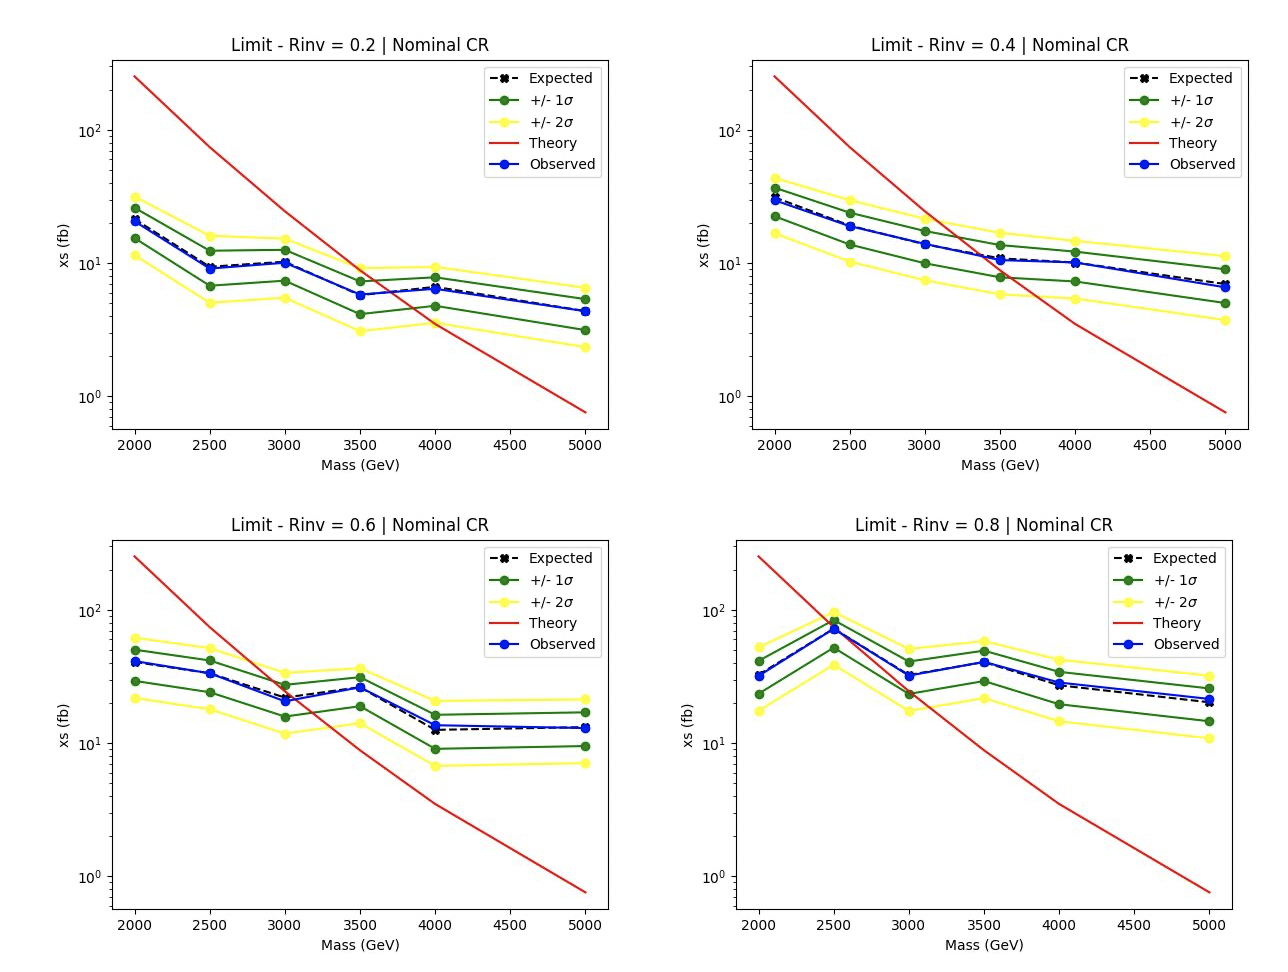
\includegraphics[width=0.95\textwidth]{figures/stats/limits_exp_1D}
    \caption{95\% C.L. upper limits on the $Z'\rightarrow q_D \bar{q_D}$ process cross section, derived from the \mt~spectrum in the CR. The red line indicates the theoretical cross section, while the blue line indicates the observed 95\% C.L. upper limit on the cross section given the data spectrum. The black line indicates the expected limit given the background shape provided by the fit. The green and yellow bands indicate the uncertainty bands. All signal models across $Z'$ mass and four different \rinv~fractions are shown. 
    \label{fig:limits_exp_1D}}
\end{figure}
%\begin{figure}[!htbp]
%\centering
%   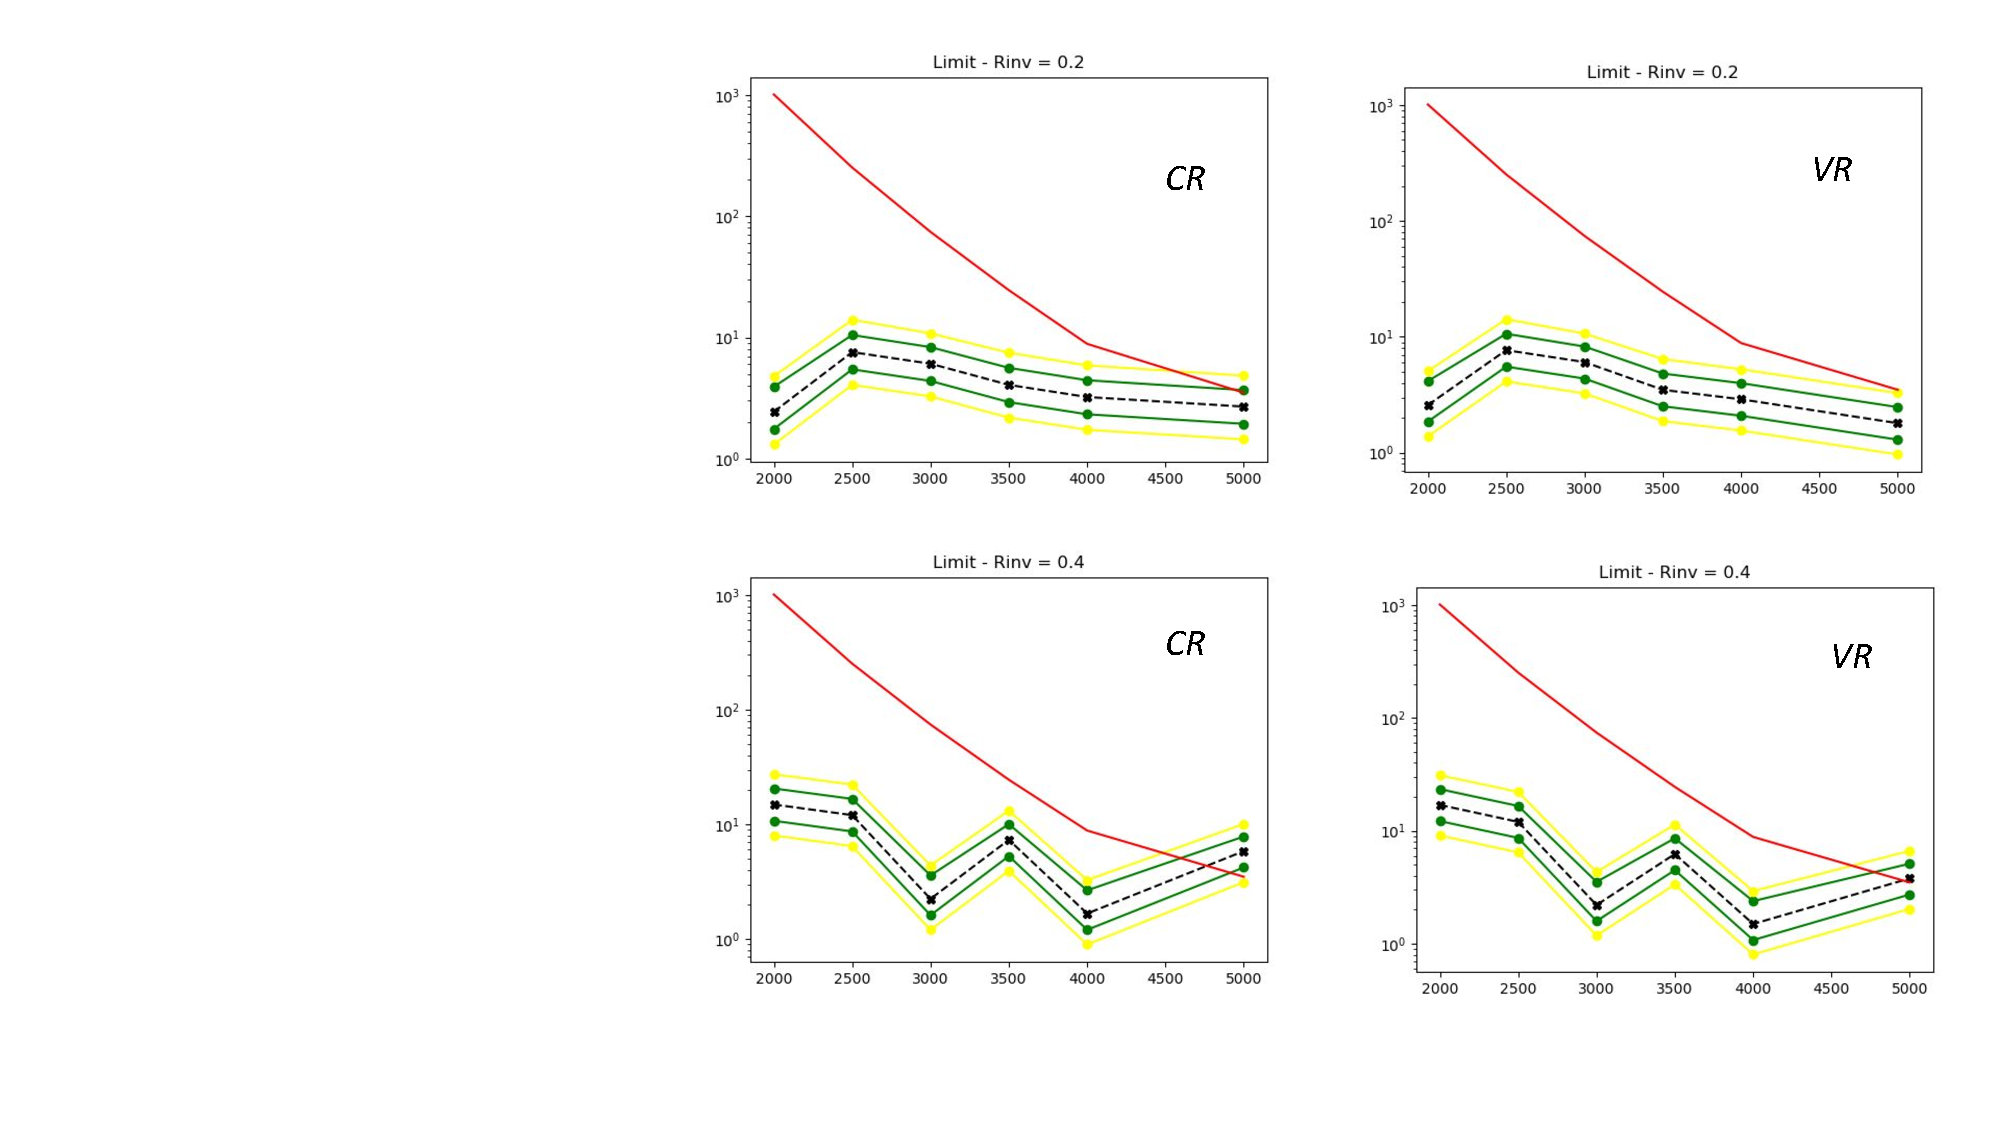
\includegraphics[width=0.9\textwidth]{figures/stats/limits_exp_1D_asimov_1}
%   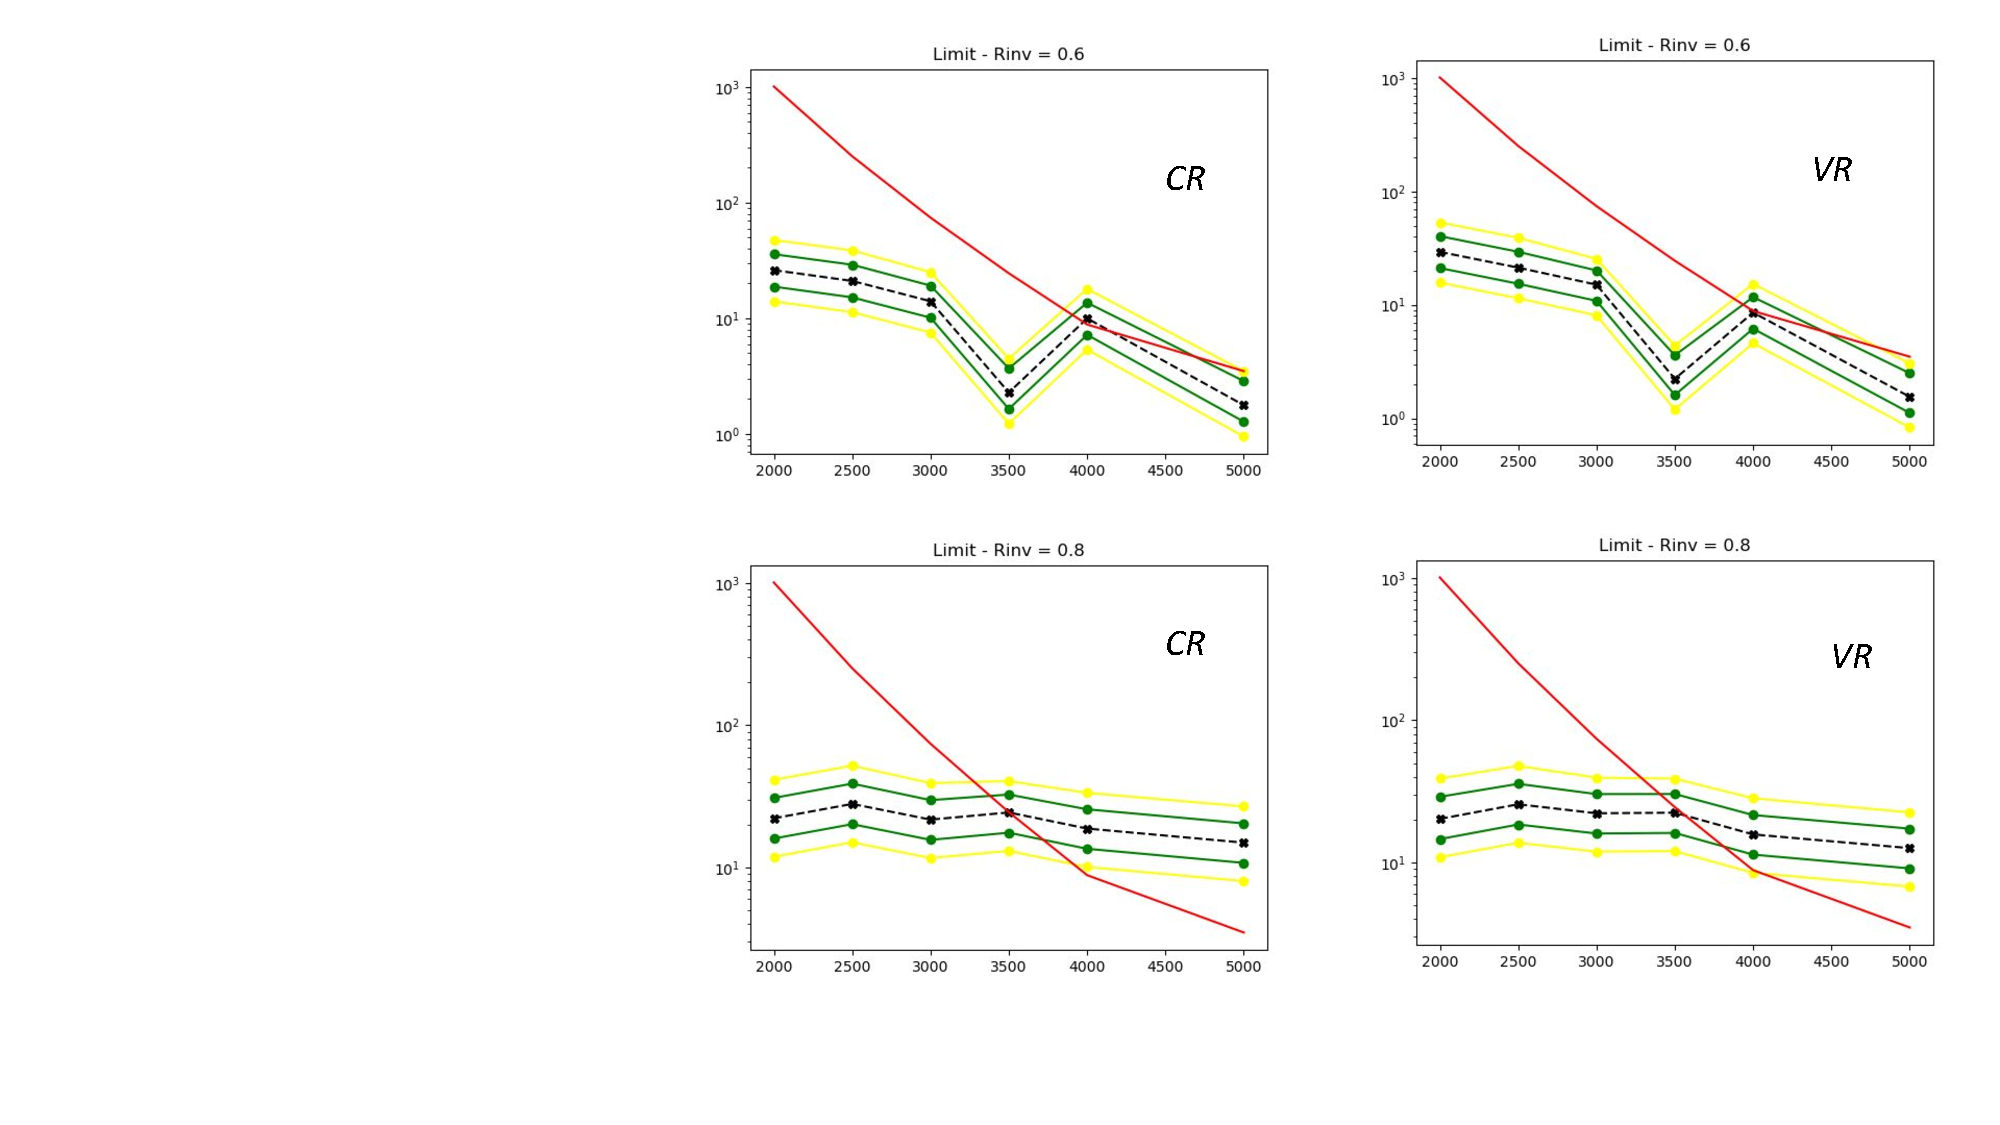
\includegraphics[width=0.9\textwidth]{figures/stats/limits_exp_1D_asimov_2}
%    \caption{95\% C.L. upper limits for signal models across Z' mass, for four different \rinv~fractions, using an average of 50 Asimov pseudo-data tests from the CR (left) and VR (right) (without systematics).
%    \label{fig:limits_exp_1D_asimov}}
%\end{figure}

%\begin{figure}[!htbp]ß
%\centering
%   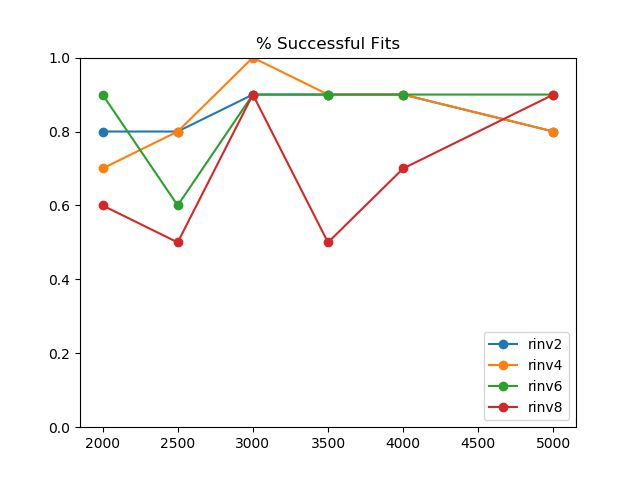
\includegraphics[width=0.6\textwidth]{figures/stats/perc_success_limit}
%    \caption{Percent of Asimov pseudodata S+B fits with successful fit and successful limit convergence.
%    \label{fig:perc_success_limit}}
%\end{figure}

The ability of the fit to identify a significant excess is tested by calculating the limits on signal injected toys. $2\sigma$ and $5\sigma$ of signal is injected for each signal point into 50 Asimov data toys.
%The number of signal events necessary for a $2\sigma$/ $5\sigma$ excess is calculated for each signal point from the expected limits in the background-only case shown in Figure~\ref{fig:limits_exp_1D}.
%The expected limit represents the limit on a $2\sigma$ excess, so a $5\sigma$ excess requires 2.5x as much signal.
Figure~\ref{fig:lim_sig_inj} demonstrates the impact of this signal injection on the limit, using signals with \rinv~= 0.2.
The observed limit rises as more signal is injected, indicating the ability of the fit to identify a significant signal excess. 

\begin{figure}[!htbp]
\centering
   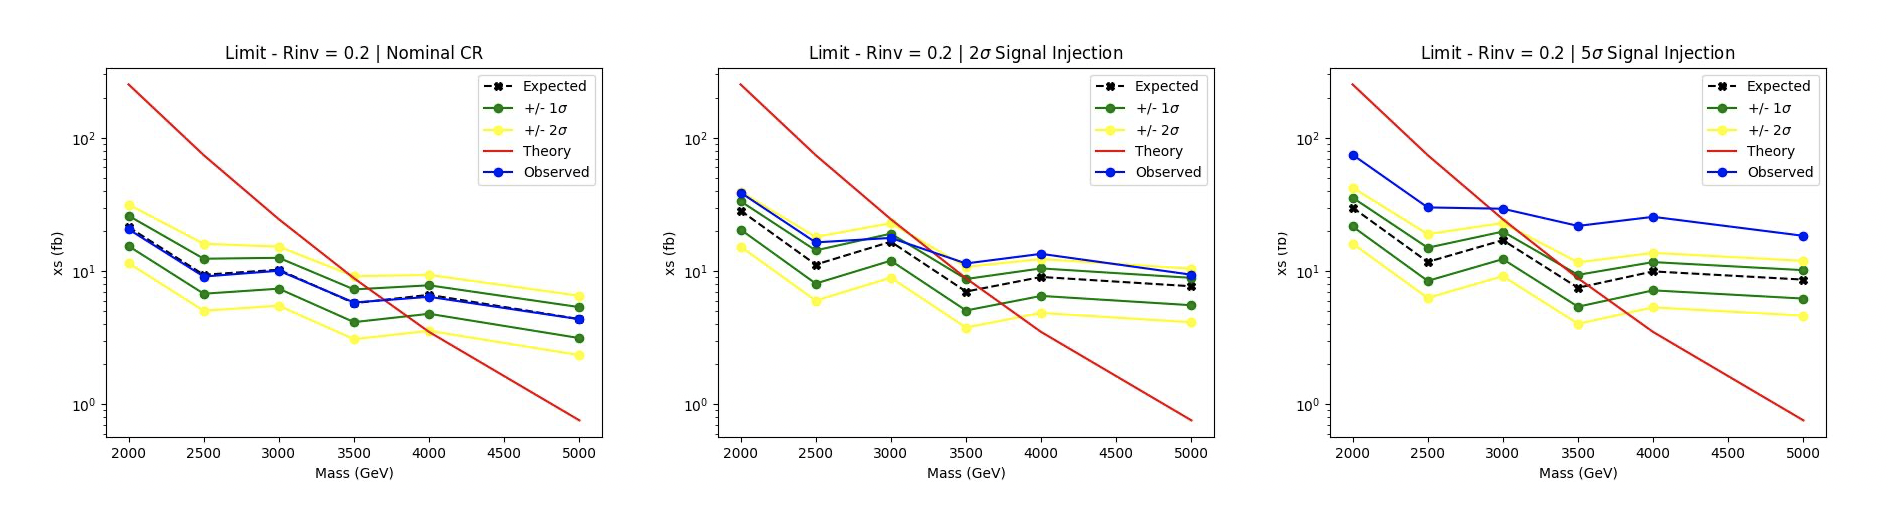
\includegraphics[width=0.98\textwidth]{figures/stats/lim_sig_inj}
    \caption{95\% C.L. observed limit for signal models across $Z'$ mass, with varying amounts of signal injected. The increasing observed limit indicates the desired behavior.
    \label{fig:lim_sig_inj}}
\end{figure}

\clearpage
